\section{Histogram with Coarse Bins}
\label{sec:coarse bin histogram}

In the Histogram with Coarse Bins we presents a parallel algorithm for histograms that does not suffer from the same serial bottlenecks as the atomic version from \cref{sec:histogram}.

The idea is to allow each block to compute their own histogram with atomic add and then use reduce to merge these histograms, which reduces steps from $\mathcal{O}(n)$ to $\mathcal{O}(\mathrm{block\_size})$.

As having a personal histogram might be memory intense giving a large amount of bins.
To avoid such we split the bins into coarse bins containing a range of bins.
Each block thus works on a coarse bin instead of the total histogram.
However, performing such coarse bin introduces a sorting of the input values according to their coarse bins.
\begin{figure}[htb]
  \centering
  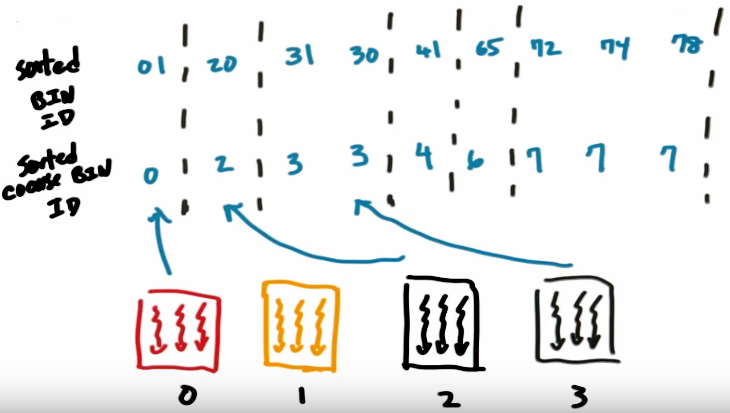
\includegraphics[width=.6\textwidth]{images/coarse-bin-example.png}
  \caption{Intuition behind coarse bin and kernel invokations}
  \label{fig:coarse bins example}
\end{figure}
The idea is illustrated in \cref{fig:coarse bins example}, where we have the sorted bin values at the top and the sorted coarse bin values at the bottom.

\
For each coarse bin histogram a \ttt{grid\_size} $\times$ the number of elements in a course bin, with \ttt{grid\_size} the number of blocks nessesary to collect all elements in the given coarse bin, is allocated as the \ttt{coarse\_bin\_grid}.
For each coarse bin a kernel is launched containing threads to gather all the elements in the coarse bin.
Each block in this kernel has its own private histogram in \ttt{coarse\_bin\_grid} in which only the given block performs updates.
At end of kernel execution the \ttt{coarse\_bin\_grid} is left with bin values represented along the columns.
In order to avoid cache misses and have coalesced access the transpose operation introduced in previous section is performed to have bin values alligned in row indexes.Given all values for each bin being set in a row we perform reduce over the rows to gather the independant block's histograms for each bin leaving an array of bin values for each coarse bin.
These are then merged resulting in the total histogram.

In our implementation we did not manage to create the full fast histogram solution as described above.
We computed the coarse bin sorting and merely had each bin atomic add to the global memory without the private \ttt{coarse\_bin\_grid} to reduce over.
From an algorithmic viewpoint this is no better than the atomic reduce histogram we were trying to improve, but it allowed us to test our coarse bin sorting.


A more detailed description of the coarse bin implementation can be found below.

Given and input array, number of bins \ttt{NUM\_BINS} and a number of coarse bins \ttt{COARSE\_SIZE} we perform the following computation.
%
\begin{enumerate}
  \item Compute bin for each value
  \item Compute coarse bin for value
  \item Sort values w.r.t. the computed coarse bins
  \item Find starting position for each coarse bin
  \item For each coarse bin --- count each bin in given range
\end{enumerate}
%
We compute the bin for each respective value as presented in \cref{lst:value bin}, where \ttt{d\_in} is the array of input values and \ttt{d\_out} is a give inputs respective bin number.

\begin{lstlisting}[caption={compute each value's bin}, label={lst:value bin}, numbers=none]
d_out[mid] = d_in[mid] % NUM_BINS;
\end{lstlisting}

Then the respective bin numbers are divided into coarse bins as presented in \cref{lst:value coarse bin}, where the \ttt{d\_in} is the array of bins, i.e. the \ttt{d\_out} from \cref{lst:value bin}.

\begin{lstlisting}[caption={compute each value's coarse bin}, label={lst:value coarse bin}, numbers=none]
d_out[mid] = d_in[mid] / COARSE_SIZE;
\end{lstlisting}

This gives an array of values, their respective bins, and their coarse bins.
The next step is to sort all the values w.r.t. the coarse bins in ascending order, i.e. coarse bin 0 is first, followed by coarse bin 1, etc.
We use the radix sort implementation we developed earlier (with slight modifications to suite our needs) to perform the sorting based on the values in the list of coarse bins.

After the values have been sorted it is possible to find the starting positions of each coarse bin.
This gives us a starting value for each coarse bin from which it is possible to calculate how many values fall into each coarse bin.
We find the positions of the bins as presented in \cref{lst:coarse bin start} by running through each value and checking if the value before it was the same value.
If the previous value is not the same then we have a starting position for the next coarse bin.

\begin{lstlisting}[caption={find the start positions of each coarse bin}, label={lst:coarse bin start}, numbers=none]
if (d_in[mid] != d_in[mid-1])
  d_out[d_in[mid]] = mid;
\end{lstlisting}

\subsection{Profiling and Analysis}

We tested and profiled our new implementation by using the \ttt{nvprof} command-line tools to get a file that could be imported into the nvidia visual profiler.
This is desirable because nvidia visual profiler is able to run a guided analysis of the program and give us advice on bottlenecks to optimize.
We computed an executable with $\mathrm{BIN\_SIZE}=100$, $n=2^{22}$ and $\mathrm{COARSE\_SIZE}=10$, which we ran with

\begin{quote}
  \ttt{nvprof --analysis-metrics -o output-file.nvprof ./executable-to-test}
\end{quote}

which gave us a file that contained all the metrics needed for the guided analysis.
This file was opened with the nvidia visual profiler and the program performed analysis of GPGPU usage.
\Cref{fig:first impl} shows the output given by the nvidia visual profiler's initial GPU usage analysis.
It informs that the algorithm has low kernel concurrency and low compute utilisation.
The low compute utilisation is mainly due to the lack of heavy lifting in our algorithm as most of our operations are memory intensive rather than computationally intensive.
As for low kernel concurrency our approach to solve the coarse bins is serial and not performed in parallel, which we could optimise upon by introducing streams.
\begin{figure}[htb]
  \centering
  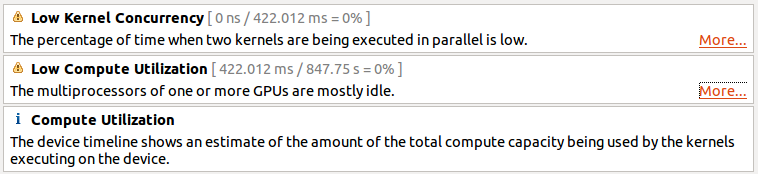
\includegraphics[width=.9\textwidth]{images/low-kernel-concurrency.png}
  \caption{NVIDIA Visual Profiler analysis}
  \label{fig:first impl}
\end{figure}

\subsection{Adding Streams}

It is possible to make kernel executions concurrent.
However, this only makes sense if the kernels are independent of each other.
So, if one or more kernels are not dependent of the output from the other kernels they can be executed concurrently.
In CUDA kernels are run concurrently with the use of streams.

Thus, from the visual profiler's analysis we tried to add streams to the kernels that were independent of the execution of the rest of the kernels.
This were the kernels that were in charge of counting and incrementing the final result of the histogram algorithm.
This modification to the code is presented in \cref{lst:coarse histo streams}.
We instantiate an array of streams and for each iteration of the loop we create a stream and invoked the kernel with it.
The full implementation is presented in \cref{ap:coarse histogram}.

\begin{lstlisting}[caption={Using streams to invoke kernels concurrently}, label={lst:coarse histo streams}]
// instantiate array of streams
cudaStream_t streams[COARSE_SIZE];

for (unsigned int i = 0; i < COARSE_SIZE; i++) {
  // create the stream for each kernel call
  cudaStreamCreate(&streams[i]);

  // set up range for local coarse bin
  local_bin_start = h_positions[i];
  local_bin_end   = (i == COARSE_SIZE-1) ? NUM_ELEMS : h_positions[i+1];

  // calculate local grid size
  amount = local_bin_end - local_bin_start;
  grid_size = amount / BLOCK_SIZE.x + 1;

  // make sure there is at least one value in coarse bin
  if (amount > 0)
    coarse_histogram_count<<<grid_size, BLOCK_SIZE, 0, streams[i]>>>(d_histogram, d_bins, local_bin_start, local_bin_end);
}
\end{lstlisting}

The resulting output did not boost the performance significantly.
We found that the sorting of the numbers used approximately $80\%$ of the execution time.
This means that the bottleneck was the sorting and not the histogram's atomic increments.
The reason for the sorting being so slow could be due to using the Hillis \& Steele scan for the compact in our radix sort implementation.
If we used the Blelloch scan instead, as debated in \cref{sec:workload and step size}, we might have been able to reduce the time spent on sorting.
